\section{Auswertung}

Zunächst muss im Versuch die Winkelrichtgröße $D$ und das
das Eigenttägheitsmoment der Drillachse $I_D$ bestimmt werden.
Anschließend die Trägheitsmoment einer Kugel und eines Zylinder (\emph{grau}).
Abschließend noch die Trägheitsmomente von einer Holzpuppe in zwei verschieden Positionen.
Da das Trägheitsmoment nicht direkt gemessen werden kann wurden immer 
die Schwingungsdauer $T$ von $5$ Schwingungen gemessen.

\subsection{Bestimmung der Winkelrichtröße $D$}

Die Winkelrichtgröße $D$ kann auf zwei verschiedene Wege bestimmt werden.
Zum einem durch eine passive und zum andern durch eien  dynamische Methode.
Beide Methoden werden im Anschluss genauer erklärt und verwendet.
Nach der Bestimmung der beiden Winkelrichtgrößen $D_{passiv}$ und $D_{dynam}$
werden diese verglichen.


\subsubsection{Passive Methode}

Die passive oder auch als statisch bezeichnete Methothde wurden mittels einem Drehmoment (gemessen mit einer Federwaage) ausgelenkt.
Wichtig dabei ist das die Federwaage immer orthogonal zum Radius steht.
Denn das Drehmoment errechnet sich mit $\vec{M}=\vec{r}\times\vec{F}$, durch 
eine orthogonale Stellung von $\vec{r}$ und $\vec{F}$ kann mit den Beträgen 
gerechnet werden und es ergibt sich der Zusammenhang $M=rF$. 
Im Versuch wurden folgende Werte bestimmt:


\begin{table}
\centering
\caption{Messung der Kraft für eine Auslenkung}
\label{tab: winkelricht}
\renewcommand{\arraystretch}{1.2}
\begin{tabular}{lcr}
	\toprule
	Abstand in $\si{\meter}$ & Winkel in $\mathrm{rad}$ & Kraft in $\si{\newton}$ \\
	\midrule
	$\num{1.01e-1}$ & $\frac{\pi}{6}$ & $\num{1.40e-1}$ \\
	$\num{1.01e-1}$ & $\frac{\pi}{3}$ & $\num{2.40e-1}$ \\
	$\num{1.01e-1}$ & $\frac{\pi}{2}$ & $\num{3.20e-1}$ \\
	$\num{1.01e-1}$ & $\frac{2\pi}{3}$ & $\num{4.60e-1}$ \\
	$\num{1.58e-1}$ & $\frac{\pi}{6}$ & $\num{6e-2}$ \\
	$\num{1.58e-1}$ & $\frac{\pi}{3}$ & $\num{1.2e-1}$ \\
	$\num{1.58e-1}$ & $\frac{\pi}{2}$ & $\num{2.20e-1}$ \\
	$\num{1.58e-1}$ & $\frac{2\pi}{3}$ & $\num{3e-1}$ \\
	$\num{2.41e-1}$ & $\frac{\pi}{6}$ & $\num{2.00e-2}$ \\
	$\num{2.41e-1}$ & $\frac{\pi}{3}$ & $\num{8.00e-2}$ \\
	$\num{2.41e-1}$ & $\frac{\pi}{2}$ & $\num{1.2e-1}$ \\
	$\num{2.41e-1}$ & $\frac{2\pi}{3}$ & $\num{2.00e-2}$ \\
	\bottomrule
\end{tabular}
\end{table}

Mit dem Zusammenhang

\begin{equation*}
D=\frac{M}{\phi}=\frac{Fr}{\phi}
\end{equation*}

ergibt sich dann für jede einzelne der $n$ Messungen ergibt sich dann ein Wert für die Winkelrichtgröße.
Diese wurden anschließend durch

\begin{equation}
\label{eq:mittel}
\bar{x}=\frac{1}{n}\sum_{i=1}x_i
\end{equation}

gemittelt, mit der dazugehörigen Abweichung

\begin{equation}
\label{eq:stand_ab}
\bar{\sigma}_{\bar{x}}=\sqrt{\frac{1}{n(n-1)}\sum_{i=1}^{n}(x_i-\bar{x})^2}.
\end{equation}

Es ergibt sich dann für damit für die Winkelrichtgröße der Wert:

\begin{equation}
\label{eq:winkel_passiv}
D_{passiv}=\left(\num{2.03e-2} \pm \num{1.22e-3}\right)\si{\newton\meter}
\end{equation}

\subsubsection{Dynamische Methode}

Bei der dynamischen Methode wurden die Schwingungsdauer von zwei kleinen Zylindern ($m_1$ und $m_2$) die symetrisch zum Mittelpunktes
eines Stabes befestigt waren gemmessen. Durch Verschiebung der Massen ergab sich eine Vielzahl von Messwerten, die im Anhang eingesehn
werden können.
Diese wurden anschließend gemittelt mit \eqref{eq:mittel} und \eqref{eq:stand_ab}.

\begin{table}
\centering
\caption{Gemittelte Schwingungsdauer für die dynamische Methode}
\label{tab: winkel_dynamisc}
%\renewcommand{\arraystretch}{1.2}
\begin{tabular}{lr}
	\toprule
	$\bar{T}$ in $\si{\per\second}$ &  $\sigma_{\bar{T}}$ in $\si{\per\second}$ \\
	\midrule
	\num{2.52} & \num{6.43e-3} \\
	\num{3.23} & \num{9.16e-3} \\
	\num{3.65} & \num{5.89e-3} \\
	\num{4.08} & \num{3.57e-3} \\
	\num{4.56} & \num{6.82e-3} \\
	\num{5.09} & \num{2.83e-2} \\
	\num{5.56} & \num{3.33e-2} \\
	\num{6.05} & \num{1.07e-2} \\
	\num{6.59} & \num{8.64e-3} \\
	\num{7.07} & \num{3.31e-3} \\
	\bottomrule
\end{tabular}
\end{table}

Mit den Schwingungsdauern und dem Gesetzt:

\begin{equation*}
T=2\pi\sqrt{\frac{I}{D}} \quad \Leftrightarrow \quad I=\frac{T^2 D}{4\pi^2}
\end{equation*}

Da die Massen von der Drehachse verschoben waren, macht man sich den Satz von Steiner \eqref{eq: steiner} zu nutze und erhält den Zusammenhang:

\begin{equation}
\label{eq:gerade}
\frac{T^2D}{4\pi^2}=I_s+ma^2\quad \Leftrightarrow \quad T^2=\frac{I_s 4\pi^2}{D}+\frac{4m_g\pi^2}{D}a^2
\end{equation}

Dabei sei $m_g=m_1+m_2=\num{222.51e-2}\si{\meter}+\num{223.46e-2}\si{\meter}$.
Offensichtlich ergibt sich eine Geradengleichung, die mit Linearer Regression angenährt werden kann.
Dazu verwendet man aus der Regressionsrechnung.

Für die Steigung $m$ ergibt sich

\begin{equation*}
m=\frac{\bar{xy}-\bar{x}\bar{y}}{\bar{x^2}-\bar{x}^2}
\end{equation*}

,mit dem dazugehörigen Fehler

\begin{equation*}
\sigma_m=\sqrt{\frac{\sigma^2}{N(\bar{x^2}-\bar{x}^2)}}.
\end{equation*}

Nach Ausführung der Regressionrechnung erhält man als Wert
\begin{equation}
\label{eq: steigung}
m=\left(\num{741.2}\pm\num{3.4}\right) \si{\kilogram\per\newton\meter}
\end{equation}

Da es sich bei \eqref{eq:gerade} um eine Gerade handelt muss gelten:

\begin{equation*}
m=\frac{4m_g\pi^2}{D}
\end{equation*}

Damit kann die Winkelrichtgröße dynamisch bestimmt werden

\begin{equation*}
D=\frac{4m_g\pi^2}{m}.
\end{equation*}

Er ergibt sich:

\begin{equation}
\label{winkelrichtgroesse_dynamisch}
D_{dynam}=\left(\num{2.38e-2} \pm \num{1.10e-4}\right)\si{\newton\meter}
\end{equation}

Da die Abweichung von $D_{dynam}$ kleiner ist als von $D_{passiv}$ wird 
diese in folgenden Rechnungen genutzt.
Dabei sie ab jetzt $D=D_{dynam}$.


\subsection{Bestimmung des Eigenträgheitsmoment $I_D$}

Auch bei der Bestimmung des Eigenträgheitsmoment machen wir uns die 
Geradengleichung \eqref{eq:gerade} und dessen Lineare Regression zunutzen.
Denn durch Betrachtung des $y$-Achsenabschnitt der Geraden kann auf das Eigenträgheitsmoment der Drillachse geschlossen werden.
Dazu

\begin{equation*}
b=\frac{4\pi^2}{D}\left(I_D+I_Z\right) \quad \Leftrightarrow \quad I_D=\frac{D}{4\pi^2}b-I_Z
\end{equation*}

Dabei sei $I_Z$ das Trägheitsmoment der kleinen Zylinder.

Aus der Regressionsrechnung ergibt sich der Zusammenhang

\begin{equation*}
b=\frac{\bar{x^2}\bar{y}-\bar{x}\bar{xy}}{\bar{x^2}-\bar{x}^2}
\end{equation*}

dür den $y$-Achsenabschnitt und der dazugehörogen Abweichung

\begin{equation*}
\sigma_b=\sqrt{\frac{\sigma^2}{N\left(\bar{x^2}-\bar{x}^2\right)}}.
\end{equation*}

Rechnerisch ergibt sich:

\begin{equation}
\label{eq:y_achsenabschnitt}
b=\left(\num{4.64}\pm\num{0.12}\right) \si{\meter}
\end{equation}

Mit dem theoretisch errechneten Wert für das Trägheitsmoment der kleinen Zylinder (mittels \eqref{eq:traeg_zylinder_schwer}) ergibt sich für das 
Eigenträgheitsmoment der Drillachse:

\begin{equation}
\label{eq:eigentraegheitsmoment}
I_D=\left(\num{0.003}\pm\num{0.000}\right) \si{\kilogram\meter\squared}
\end{equation}


Abschließend wird der schon benutzte lineare Zusammenhang zwischen $T^2$ und $a^2$ graphisch aufgezeigt.

\begin{figure}
  \centering
  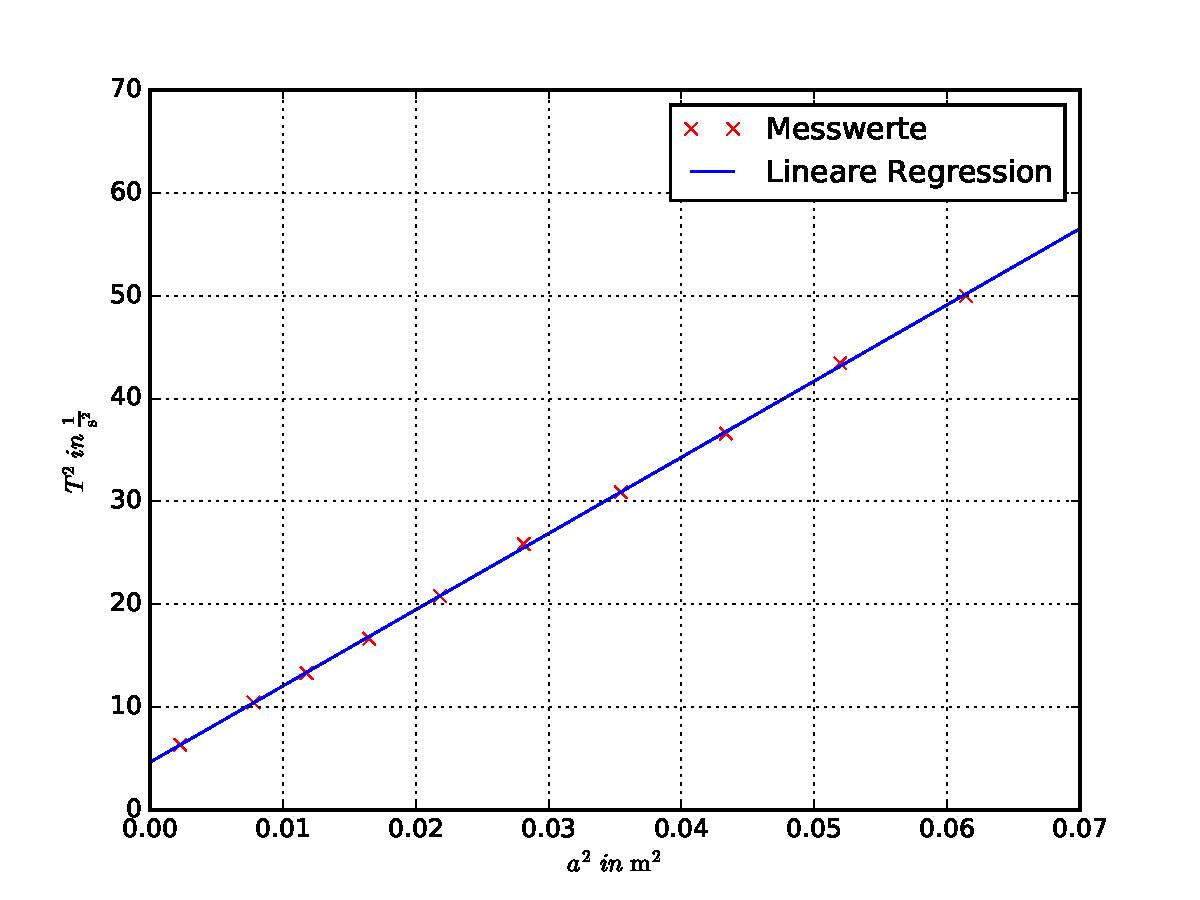
\includegraphics[width=0.9\textwidth]{pics/lineare_regression.pdf}
  \caption{Zusammenhang zwischen $T^2$ und $a^2$}
  \label{fig:zusammenhang_a_T}
\end{figure}


\subsection{Experimentelle Bestimmung des Trägheitsmoment von Zylinder und Kugel}

Um das Trägheitsmoment zu bestimmen wird der Zusammenhang

\begin{equation*}
I_{körper}=\frac{T^2 D}{4\pi^2}-I_D
\end{equation*}
genutzt.
Am Ende jedes Unterkapitel soll ein Vergleich mit den
Trägheitsmomenten erfolgen die sich aus der Theorie ergeben.

\subsubsection{Trägheitsmoment des Zylinder}

Die gemessenen Schwingungsdauer sind im Anahng nachzulesen.
Als gemittelter Wert ergibt sich:

\begin{equation*}
\bar{T}_{zylin}=\left(\num{1.17}\pm\num{0.00}\right) \si{\per\second}
\end{equation*}

Damit folgte für das Trägheitsmoment:

\begin{equation}
\label{eq:traeg_zylinder_grau_exp}
I_{zylin}=\left(\num{0.0008}\pm\num{0.0000}\right) \si{\kilogram\meter\squared}
\end{equation}

Für die theoretische Berechnung werden die Maße und Masse des Zylinders benötigt. Sie lauten:

\begin{align*}
\text{Maße} \quad &\\
d&=\num{3.49e-2}\si{\meter}\\
h&=\num{3.01e-2}\si{\meter}\\
\text{Masse} \quad &\\
m_{zyl}&=\num{1005.8}\si{\gram}
\end{align*}

Da es sich hier um eine Drehung um die Symetrieachse handelt wird zu
theoretischen Berechnung \eqref{eq:traeg_zylinde} genutzt.
Das resultierende Ergebnis lautet:

\begin{equation}
\label{eq:traeg_zylinder_theo}
I_{zylin \,theo}= \num{0.0006}\si{\kilogram\meter\squared}
\end{equation}

Die Abweichung vom experiementell Resultat zur Theorie beläuft sich auf $\approx +33 \%$

\subsubsection{Trägheitsmoment der Kugel}

Bei der Bestimmung des Trägheitsmoment einer Kugel wurde genauso Vorgegangen wie bei 
der Bestimmung für den Zylinder. Auch hier sind die gemessenen Schwingungsdauer im Anhang einzusehen.
Als gemittelter Wert ergibt sich:

\begin{equation*}
\bar{T}_{kugel}=\left(\num{1.66}\pm\num{0.00}\right) \si{\per\second}
\end{equation*}

Daraus folgt für das Trägheitsmoment:

\begin{equation}
\label{eq:traeg_kugel_exp}
I_{kugel}=\left(\num{0.002}\pm\num{0.000}\right) \si{\kilogram\meter\squared}
\end{equation}

Um das theoretische Trägheitsmoment zu bestimmen werden die Abmessungen und das Gewicht der Kugel benötigt:

\begin{align*}
\text{Abmessung} \quad &\\
d&=\num{13.78e-2}\si{\meter}\\
\text{Gewicht} \quad &\\
m_{zyl}&=\num{812.40}\si{\gram}
\end{align*}

Als theoretische Grundformel wird \eqref{eq:traeg_kugel} genutzt.
Es resultiert 

\begin{equation}
\label{eq:traeg_kugel_theo}
I_{kugel \,theo}= \num{0.002}\si{\kilogram\meter\squared}
\end{equation}

als theoretishes Trägheitsmoment.

Aschbließend gilt es noch zu erwähnen das es keinen unterschied
zwischen theoretischen und experiementell Trägheitsmoment gibt.

\subsection{Trägheitsmoment der Modellpuppe}

Wie auch bei den voherigen Körpern wird zu Bestimmung des Trägheitsmoment
die Schwinugngsdauer der Puppe gemessen.

Der wesentliche Unterschied zu den vohrigen Körpern ist der Vergleich mit den theoretischen Werte. Den beid er Berrechnung muss die Form der Puppe 
durch bekannkte Körper (Zylinder und Kugeln) angenährt werden.
Da die einzelnen Körperteile nicht an jeder Stelle die gleichen Maße haben,
wurde mehere Werte gemessen (siehen Anhang) und dann gemittelt.
Das Ergebnis sind folgende Abmessungen für die Puppe:

\begin{align*}
\text{Abmessung} \quad &\\
r_{kopf}&=\left(\num{0.027}\pm\num{0.002}\right)\si{\meter}\\
r_{arm}&=\left(\num{0.015}\pm\num{0.001}\right)\si{\meter}\\
r_{torso}&=\left(\num{0.035}\pm\num{0.004}\right)\si{\meter}\\
r_{bein}&=\left(\num{0.018}\pm\num{0.001}\right)\si{\meter}\\
\text{Gewicht} \quad &\\
m_{puppe}&=\num{161.90}\si{\gram}
\end{align*}

Für spätere berechnung wurde die Puppe wie auf der folgenden Abbildung zusehen geometrisch angenährt:


\begin{figure}
  \centering
  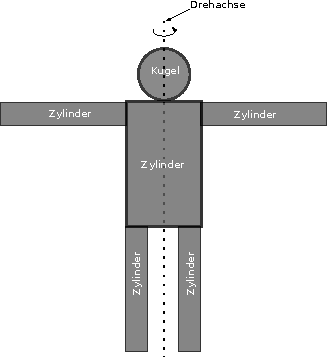
\includegraphics[width=0.6\textwidth]{pics/puppe.pdf}
  \caption{Annäherung der Puppe}
  \label{fig:approx_puppe}
\end{figure}

\subsubsection{Position 1}

Die Haltung der Puppe in Position 1 ist in Abbildung \ref{fig:pup1} dargestellt.
Die gemessenen Schwingungsdauer sind im Anahng aufgelistet.
Als Mittelwert ergibt sich:

\begin{equation*}
\bar{T}_{puppe\, p1}=\left(\num{0.64}\pm\num{0.00}\right) \si{\per\second}
\end{equation*}

Daraus resultultier für das Trägheitsmoment:

\begin{equation}
\label{eq:traeg_puppe_p1}
I_{puppe \,p1}= \left(\num{0.0002}\pm\num{0.0000}\right)\si{\kilogram\meter\squared}
\end{equation}

Bei der Berechnung des theoretischen Trägheitsmoment, macht man sich das additives Verhalten der Trägheitsmomente zu nutzen.
Dabei ist jeodch zu beachten, das bei den Armen und Beinen der Satz von Steiner zu berücksichtigen sind. Dabei sind die Verschiebungen zur Drehachse
\begin{align*}
a_{arm}&=\num{9.27e-2}\si{\meter}\\
a_{bein}&=\num{1.19e-2}\si{\meter}
\end{align*}

Desweiteren wird für den Satz von Steiner die Masse von Arm und Bein benötigt.
Diese werden bestimmt indem man das Teilvolumen von Arm und Bein zum Gesamtvolumen bestimmt. Das Teilvolumen wird dann anschließend mit der Masse der Puppe multipliziert.

Für den Arm ergab sich
\begin{align}
\begin{aligned}
\label{eq:masse_arm}
\text{prozentualer} Anteil \quad &\left(10\pm\num{1}\right)\% \\
\text{Masse Arm} \quad &\left(\num{0.016}\pm\num{0.002}\right)\si{\kilogram}
\end{aligned}
\end{align}

und für ein Bein

\begin{align}
\begin{aligned}
\label{eq:masse_bein}
\text{prozentualer} Anteil \quad &\left(16\pm\num{2}\right)\% \\
\text{Masse Bein} \quad &\left(\num{0.026}\pm\num{0.003}\right)\si{\kilogram}.
\end{aligned}
\end{align}

Nach der Theorie hat die Puppe in Position $1$ ein Trägheitsmoment von

\begin{equation*}
\bar{T}_{puppe\, p1\,theo}=\left(\num{1.55e-5}\pm\num{0.27e-5}\right) \si{\kilogram\meter\squared}.
\end{equation*}

Der Unterschied zwischen Theorie und Praxis liegt bei $\approx +1200 \%$.

\subsubsection{Position 2}
Die Haltung der Puppe in Position 2 ist in Abbildung \ref{fig:pup2} zusehen.
Die gemessenen Schwingungen sind im Anhang abgedruckt.
Als gemittelte Schwingungsdauer errechnet sich:

\begin{equation*}
\bar{T}_{puppe\, p2}=\left(\num{0.91}\pm\num{0.00}\right) \si{\per\second}
\end{equation*}

Damit folgt für das Trägheitsmoment

\begin{equation}
\label{eq:traeg_puppe_p2}
I_{puppe \,p2}= \left(\num{0.0005}\pm\num{0.0000}\right)\si{\kilogram\meter\squared}
\end{equation}

Da bei dieser Position nur die Beine ihre Position geändert haben, ändert sich auch nur ihr Abstand zu Drehachse auf $a=\num{6.77e-2}\si{\meter}$.
Sonst bleiben Massen und Abstände gelich.

Für das theoretische Trägheitsmoment folgt

\begin{equation*}
\bar{T}_{puppe\, p2\,theo}=\left(\num{0.0002}\pm\num{0.0000}\right) \si{\kilogram\meter\squared}.
\end{equation*}

Die Abweichung von der experimentellen und theoretischen Messung ist 
somit $\approx +250 \%$.


